\documentclass[a4paper,12pt]{article}
\usepackage[utf8]{inputenc}
\usepackage[T1]{fontenc}
\usepackage[spanish]{babel}
\usepackage{csquotes}
\usepackage{anysize}
\usepackage{graphicx}
\marginsize{25mm}{25mm}{25mm}{25mm}

\title{The paradoxical effect of low reward probabilities in suboptimal choice}
\author{Inês Fortes, Carlos Pinto, Armando Machado,\\ Marco Vasconcelos}
\date{2018}

\begin{document}

{\scshape\bfseries \maketitle}

La atención de los animales a los eventos ambientales es selectiva y dinámica, y se basa en lo que es más importante para el organismo en cada momento. Estudiar instancias en que los animales parecen ignorar eventos importantes podría informarnos sobre los límites de los procesos conductuales. En elección subóptima los animales hacen justo eso al elegir la alternativa informativa sobre la no informativa: parecen ignorar las consecuencias negativas de la alternativa informativa.

Algunos modelos (como {\itshape Reinforcement Rate Model} y {\itshape Hyperbolic Discounting Model}) asumen que las palomas ignoran al estímulo discriminativo negativo $S_{Green,0{.}0}$, comportándose como si nunca se presentara, por lo que subjetivamente para ellas la opción informativa lleva siempre a $S_{Red1{.}0}$ y tiene una tasa mayor de reforzamiento que la no informativa. Esta idea es apoyada por experimentos en los que se altera la duración o la probabilidad de $S_{Green0{.}0}$ hasta un máximo de 200 segundos sin que haya grandes cambios en la preferencia.

¿Cómo se relaciona la probabilidad de atender a un estímulo con la probabilidad de que éste anuncie la entrega de comida? Si se aumenta de 0 a $p$ la probabilidad de entrega de comida de $S_{Green0{.}0}$, ¿la atención incrementaría súbitamente o de forma gradual? ¿El cambio en la atención cambiaría la preferencia? Al atender, el animal queda expuesto tanto a los aspectos positivos de atender (las recompensas) como a los negativos (los tiempos muertos), y la valoración conjunta de ambas consecuencias debería determinar el valor de la alternativa.

La meta del artículo es ver cómo cambia el valor de la alternativa informativa según se va incrementando la probabilidad de reforzamiento de $S_{Green}$. Las predicciones son contraintuitivas: suponiendo que (a) los animales atienden a $S_{Green}$ siempre que la probabilidad de reforzamiento $p > 0$, (b) escogen la opción con la tasa de reforzamiento percibida más alta, y (c) esto último es igual a la tasa entre la probabilidad de reforzamiento promedio asociada con esa opción y la duración percibida de su terminal link; la tasa de reforzamiento percibida para la alternativa no informativa es independiente de $p$ y es igual siempre a 0.05 recompensas/s (es decir, $\frac{0.5}{0.5\times10+0.5\times10}$). Mientras, la tasa percibida de la alternativa informativa es dependiente de $p$: cuando $p=0$, los animales no atienden a $S_{Green}$ y por lo tanto no consideran su duración. Así, la tasa de reforzamiento percibida para la alternativa informativa es de 0.10 recompensas/s (es decir, $\frac{0.2}{0.2\times10+0.8\times0}$). En esta condición, los animales deberían preferir la alternativa informativa, predicción que es consistente con los resultados hasta ahora. 

Sin embargo, cuando $p$ incrementa a 0.1, los animales atienden a $S_{Green}$ con sus costos y sus beneficios, con lo que la tasa de reforzamiento percibida se vuelve 0.028 recompensas/s (es decir, $\frac{0.2\times1+0.8\times0.1}{0.2\times10+0.8\times10}$). Dado que ahora esta tasa es menor que aquella de la alternativa no informativa, los animales deberían revertir su preferencia. La predicción es contraintuitiva porque implica que la preferencia por la alternativa informativa disminuye cuando aumenta su probabilidad de reforzamiento.

Cuando $p$ incrementa a 0.375, entonces la tasa percibida se vuelve 0.05 e iguala a la tasa de la alternativa no informativa. Con eso, la preferencia debería revertirse una vez más. Aunque aun no se sabe si los animales atenderán a $S_{Green}$ en cualquier $p > 0$.

Los presentes experimentos pretenden probar esas predicciones y examinar cómo cambia la preferencia con $p$. En el experimento 1 se varió $p$ entre fases y se midió el valor relativo de las dos opciones mediante la proporción de elección en los IL. En el experimento 2 se varió $p$ entre fases, pero intra fase se cambió la demora en los eslabones terminales de la opción no informativa. Se midió el valor relativo de las opciones mediante la duración $D$ que hacía a las palomas indiferentes entre los dos IL.

{\scshape\bfseries Experiment 1: Probability of Food on the Informative Option}

{\scshape\bfseries Procedure}

Las sesiones tenían 120 ensayos: 40 libres y 80 forzados. Las probabilidades de presentación de los estímulos eran de .2 y .8, y los estímulos eran $S_{Red1{.}0},\ S_{Green0{.}0},\ S_{Yellow0{.}5}$, y $S_{Blue0{.}5}$. 

El 80\% de los ensayos de la alternativa informativa terminaba en $S_{Green,p}$. Las probabilidades de reforzamiento que seguían a $S_{Green,p}$ se manipularon entre sujetos en los valores de $p = 0/32, 1/32, 6/32, 12/32$. Sin importar la probabilidad de reforzamiento de $S_{Green,p}$, su estímulo complementario $S_{Red1{.}0}$ continuaba entregando confiablemente reforzamiento, con lo que en el caso de $p= 12/32$ la probabilidad global de reforzamiento subió hasta 0.5. 

{\scshape\bfseries Results and Discussion}

Las palomas adquirieron una fuerte preferencia por la alternativa informativa al final de sus 15 sesiones en todos los grupos.

\begin{figure}[ht]
	\begin{center}
		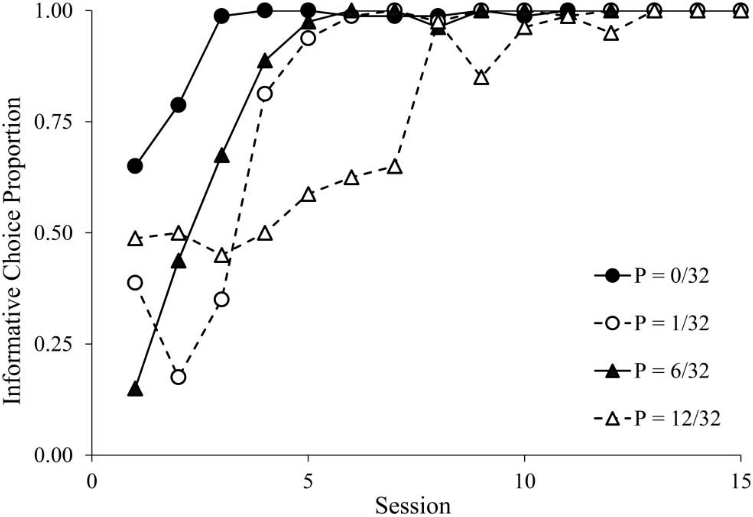
\includegraphics[scale=0.3]{Fortes2018.png}
	\end{center}
\end{figure}

Esto puede explicarse por el hecho de que incrementar $p$ incrementa la probabilidad global de reforzamiento de la alternativa informativa. Sin embargo, aunque la preferencia sea la misma, eso no significa que el valor lo sea. Puede ser que, en el rango probado, la alternativa informativa continuó siendo más valiosa que la no informativa.

Hay evidencia débil que muestra que la tasa de adquisición de la preferencia se hizo más lenta con el incremento en $p$. Esto significaría que (1) mientras $p$ incrementaba, la probabilidad de reforzamiento de la alternativa informativa se aproximaba a la no informativa (.2, .225, .35 y .5 vs .5). Si la probabilidad global afecta a la conducta, la adquisición más lenta podría deberse a un incremento en la dificultad para discriminar las probabilidades de cada alternativa. O (2) el decremento en la tasa de adquisición podría significar que cuando incrementa $p$, el valor subjetivo de la alternativa informativa disminuye paradójicamente, aproximándose al valor de la no informativa.

Un efecto de techo pudo haber ocultado las diferencias entre los valores de la alternativa informativa entre grupos. Para ello se propuso el segundo experimento 2, que estaba diseñado para probar empíricamente si el valor de una opción preferida incrementa o decrementa cuando ésta es más a menudo recompensada.

{\scshape\bfseries Experiment 2: Probability of Food on the Informative Option With Reduced Delays on the Noninformative Option}

Un método alternativo para medir el valor de la alternativa informativa es incrementar el valor de la alternativa no informativa y comparar en qué punto los sujetos son indiferentes entre las dos. En el experimento 2 se manipuló sistemáticamente la demora del TL de la alternativa no informativa. Mientras  las demoras decrementan, la opción no informativa debería hacerse más atractiva, causando que la preferencia por la alternativa informativa se revierta. Al incrementar las demoras, la preferencia por la alternativa informativa debería aumentar.

Este decremento e incremento de preferencia por la opción informativa debería ser una función de $p$. Si incrementar $p$ incrementa el valor de la alternativa informativa, entonces cuanto más grande sea $p$ más debería tardar en disminuir la preferencia (es decir, la preferencia debería necesitar un gran decremento en el TL de la alternativa no informativa para revertirse, un incremento pequeño para volver a aumentar). Si $p$ disminuye el valor de la alternativa informativa, entonces cuanto mayor sea $p$ más pronto debería revertirse la preferencia y más debería tardar en recuperarse.

{\scshape\bfseries Procedure}

El procedimiento fue el mismo con las siguientes diferencias: comenzó con 80 ensayos aleatorios forzados y terminó con 80 de elección. Todas las duraciones de TL comenzaron en 20s en lugar de 10s. Las duraciones de TL de la opción no informativa decrementaron e incrementaron sistemáticamente. Decrementaron de 20 a 0 en pasos de 4s, y luego incrementaron de 0 a 20.

{\scshape\bfseries Results and Discussion}

Las aves continuaron prefiriendo la alternativa informativa cuando los TL incrementaron a 20s. Según decreció la duración de los TL de la alternativa no informativa, todas las aves cambiaron su preferencia hacia ella, y cuando los TL incrementaron de nuevo, la preferencia reemergió.

\begin{figure}[ht]
	\begin{center}
		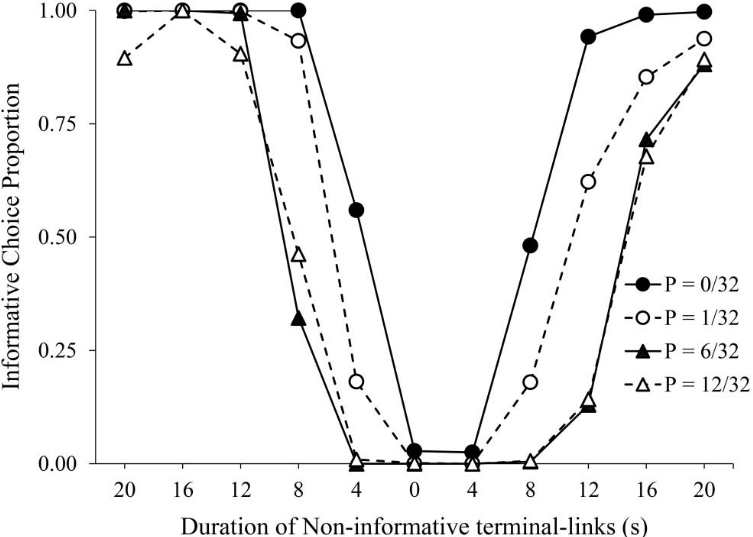
\includegraphics[scale=0.3]{Fortes2018(2).png}
	\end{center}
\end{figure}

Según disminuyó la duración del TL, la preferencia por la alternativa informativa disminuyó primero para los grupos con una mayor probabilidad de reforzamiento asociado con $S_{Green,p}$($p=6/32$ y $p=12/32$), luego para el grupo $p=1/32$, y finalmente para el grupo de $p=0/32$. Después, cuando la demora del TL incrementó, la preferencia por la alternativa informativa incrementó primero para $p=0/32$, luego $p=1/32$, y finalmente para $p=6/32$ y $p=12/32$. Esta simetría en la función de elección es confirmada por la correlación positiva entre los puntos de indiferencia calculados con los datos ascendentes y descendentes. La curva tiene un leve sesgo hacia la derecha, lo que sugiere un efecto de acarreo producido por las duraciones previas de los TL de la alternativa no informativa.

Para estimar el punto de indiferencia se promediaron los puntos de indiferencia ascendente y descendente. Hubo un efecto significativo de la probabilidad de reforzamiento sobre los puntos de indiferencia, y hubo diferencias significativas entre el grupo $p=0/32$ y los grupos $p=6/32$ y $p=12/32$.

Cuando $p=0/32$, la alternativa informativa proveía 2.5 veces menos reforzamiento que la no informativa, y aun así era preferida. La preferencia solo se revirtió cuando la duración del TL de la alternativa no informativa se redujo en un 70\%. En el otro extremo, en el grupo de $p=12/32$ ambas opciones entregaban comida en el 50\% de las ocasiones, pero el TL de la opción no informativa debió reducirse en un 41\% para que los animales revirtieran su preferencia. Esto significa que aunque la opción informativa entregaba más comida para el grupo $p=12/32$ que para el grupo $p=0/32$, el primer grupo requirió un decremento más pequeño en el TL de la alternativa no informativa para revertir su preferencia. Esto sugiere que el valor de la alternativa informativa {\itshape disminuyó} cuando incrementó su probabilidad de reforzamiento $p$.

{\scshape\bfseries General Discussion}

La meta del experimento era medir cómo cambiaba el valor de la alternativa informativa mientras aumentaba su probabilidad de reforzamiento $p$. La premisa era que la preferencia subóptima se da porque, una vez aprendida la tarea, los animales no le prestan atención al estímulo que predice la ausencia de comida $S_{Green,0{.}0}$. Así, la alternativa informativa subjetivamente siempre entrega comida. Al incrementar su probabilidad de reforzamiento se esperaba que las palomas comenzaran a involucrarse con el estímulo, e interesaba saber cómo eso afectaría al valor de la alternativa informativa.

En el experimento uno se expuso a cuatro grupos a probabilidades de reforzamiento distintas en la alternativa informativa. Todos la prefirieron, sin embargo el efecto de techo ocultó el cambio en el valor dado por el cambio en $p$. En el experimento dos se encontró evidencia de que, paradójicamente, cuanto más reforzamiento se entrega siguiendo a $S_{Green,p}$, menos valor tiene la alternativa.

{\scshape\bfseries Theoretical Implications}

Para determinar si los modelos existentes de elección subóptima pueden ajustarse a estos resultados es necesario especificar la {\itshape engagement function}, $f$, que relaciona la probabilidad de reforzamiento de un estímulo, $p$, con la probabilidad de involucrarse con él, $f(p)$. Se asume que $f(0)=0$ (el animal no atiende a $S_{Green,0{.}0}$), y $f(1)=1$ (el animal siempre atiende a $S_{Red,1{.}0}$), pero una forma más general no se ha especificado.

Se examinan dos candidatos para $f(p)$: una función todo-o-nada y una función lineal. Además de la función, para predecir la elección se requiere conocer cómo los costos y beneficios de involucrarse con dos o más estímulos de TL se combinan para determinar el valor de un estímulo de IL. Para esto se toman los modelos de elección.

Modelos funcionales como el Reinforcement Rate Model (RRM) enfatizan cómo la selección natural actúa sobre la adecuación de las estrategias de forrajeo (causas últimas). Modelos mecanísticos como el HDM se enfocan en los procesos psicológicos que guían la conducta (causas proximales).

Según el RRM, cuando los animales encuentran una elección, escogen la opción que maximiza la tasa de ingesta de energía computada como la razón entre ganancia esperada y tiempo gastado para obtener la comida. Pero en esta computación no se consideran todas las duraciones: cuando un estímulo nunca va seguido de reforzamiento, se ignora. De forma similar, el HDM asume que un estímulo no seguido por reforzamiento no se convierte en un reforzador condicionado y es ignorado por los animales. la pregunta de interés es si estos modelos pueden capturar la modulación del valor de la alternativa informativa cuando $S_{Green}$ es reforzado ocasionalmente.

La función todo-o-nada asume que si un estímulo es seguido por reforzamiento con una probabilidad mayor que un umbral, generará involucramiento. De lo contrario, no.  La función lineal asume que la verosimilitud de que el animal se involucre con un estímulo es determinada por la probabilidad de reforzamiento del estímulo: a mayor reforzamiento, mayor verosimilitud de que el animal se involucre.

Se incluye la función todo o nada en el RRM.
$$
f(p) = \left\{\begin{array}{ll}
		0,&p\leq\Theta\\
		1,&p>\Theta
	\end{array}
	\right.
$$
Es decir, habrá involucramiento solamente si $p$ supera al umbral $\Theta$.

Se asume que si $p$ es menor que un umbral $\Theta$, entonces el animal ignorará a $S_{Green}$ y se encontrará subjetivamente en una situación en la cual la alternativa informativa siempre entrega reforzamiento. Si $p>\Theta$, entonces el animal atenderá a $S_{Green}$, y por lo tanto se verá influido por su probabilidad de reforzamiento. Asumiendo que la probabilidad de reforzamiento de la alternativa no informativa es de 0.5 y que $\Theta=0.1$, los animales deberían tener tres políticas de respuesta distintas:

\begin{enumerate}
	\item Mientras $p\leq\Theta$, dado que se encuentran subjetivamente en una situación en la que la alternativa informativa siempre entrega reforzamiento, deberían preferirla, pues la no informativa solo lo entrega en la mitad de las ocasiones.
	\item Mientras $\Theta \leq p \leq 0{.}375$ los animales deberían preferir la alternativa no informativa, en tanto que ya se involucran con el estímulo negativo de la alternativa informativa y ésta tiene una menor densidad de reforzamiento que la alternativa no informativa.
	\item Mientras $p > 0{.}375$ los animales deberían revertir su preferencia de vuelta hacia la alternativa informativa puesto que ahora tiene una  mayor densidad de reforzamiento que la no informativa.
\end{enumerate}

En cambio, con una función lineal de involucramiento la probabilidad de reforzamiento después de un estímulo determina la verosimilitud de que el animal se involucre. La única función lineal que satisface las condiciones asumidas de $f(0)=0$ y $f(1)=1$ es 
$$
f(p)=p
$$
Con esto, el animal solo se involucra en la alternativa no informativa en la mitad de los ensayos y por lo tanto solo toma en cuenta la mitad de los reforzadores y demoras que tiene asociados. El valor de la alternativa no informativa permanece igual ya sea que la función de involucramiento sea todo-o-nada o lineal.

El valor de la alternativa informativa cambia de forma no lineal con $p$. Mientras $p$ aumenta y crece la probabilidad global de reforzamiento de la alternativa, su valor sigue una forma de U con un mínimo en $p\approx {.}31$. Para toda $p$ la alternativa informativa tiene un valor mayor que la no informativa, por lo que se predice preferencia por la informativa.

En resumen, con una función lineal de involucramiento se predice preferencia por la alternativa informativa sin importar la probabilidad de reforzamiento en $S_{Green}$. Si la regla de decisión es {\itshape winner-takes-all}, los animales deberían preferir exclusivamente la alternativa informativa. Pero con una regla menos extrema la proporción de elección debería estar por encima de .5, pero debería tener una forma similar al valor de la alternativa informativa en

\begin{figure}[ht]
	\begin{center}
		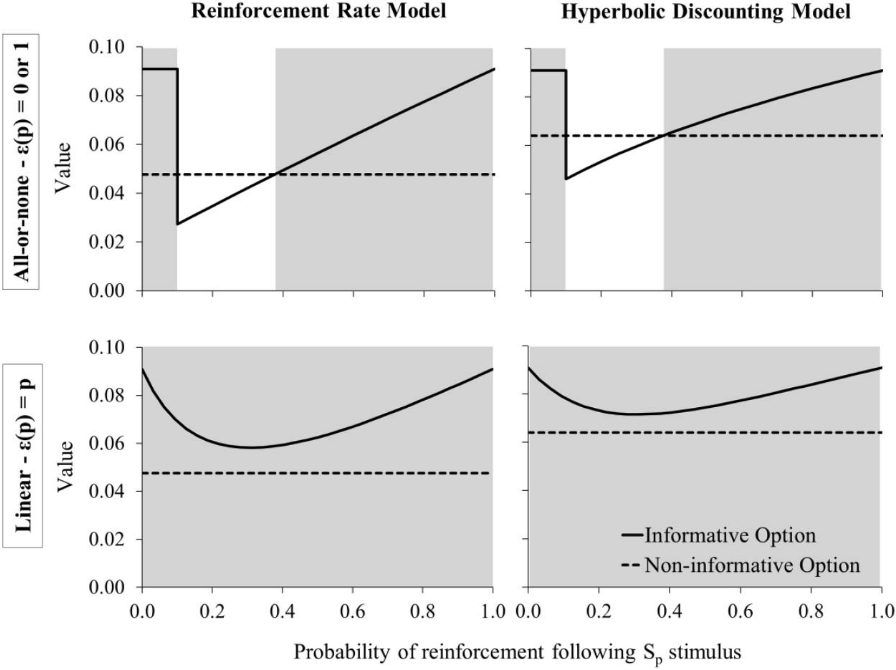
\includegraphics[scale=0.4]{Fortes2018(3).png}
	\end{center}
\end{figure}

Es decir, una preferencia más fuerte por la alternativa informativa en los valores más altos y más bajos de $p$, y valores cercanos a la indiferencia en valores de $p$ intermedios.

\newpage
Pasando al Hyperbolic Discounting Model, el valor de una recompensa demorada está dado por 
$$
V=\frac{A}{1+KD}
$$
donde $V$ es el valor, $A$ se relaciona con la cantidad de la recompensa, $D$ es la demora, y $K$ es un parámetro de descuento.

Según el HDM, un reforzador probabilístico es funcionalmente equivalente a un conjunto de reforzadores entregados tras distintas demoras siempre que estas demoras incluyan solo el tiempo pasado en presencia de un estímulo que sea al menos parcialmente reforzado. Es decir, estímulos nunca seguidos por recompensas son ignorados y excluídos de los cálculos. Un animal que se enfrenta a los esímulos A y B que entregan recompensas probabilísticas llega a tres posibles eventos: $A^+$, el animal atiende y es reforzado; $A^-$, el animal atiende pero no es reforzado; y $A^0$, el animal no atiende (lo mismo para B).

De manera similar al RRM, al integrar la función todo o nada en la ecuación del HDM el resultado indica tres distintas políticas en los mismos puntos. Y al integrar la función lineal se obtiene el mismo comportamiento que con RRM (preferencia por la alternativa informativa sin importar la $p$), aunque con un valor más elevado.

La diferencia principal entre las funciones de involucramiento es que la todo-o-nada predice una reversión de la preferencia, mientras que la lineal no. Sin embargo, la sola preservación de la preferencia no es suficiente para concluir que la función es lienal: es necesario demostrar que aunque la preferencia se mantuvo, el valor de la alternativa informativa disminuyó con aumentos en $p$.

Justo eso es lo que apoyan los datos: los resultados del experimento 2 indican que cuanto más se refuerza un estímulo, más se le atiende, y esta atención incrementa de forma lineal y no con base en un umbral.

Ambos modelos (RRM y HDM) mostraron predicciones relativamente acertadas en cuanto a los puntos de indiferencia: tenían la tendencia correcta, pero sobreestimaban el punto.

Una explicación alternativa de los datos puede venir de la teoría de la información: según ella, cuanta más incertidumbre de recompensa tiene asociado un estímulo, menos valor tiene. Así, un estímulo con probabilidad de reforzamiento de 0 o 1 tiene mínima incertidumbre y valor máximo, y un estímulo con probabilidad de 0.5 tiene lo contrario. En este experimento al aumentar la probabilidad de reforzamiento de $S_{Green}$ se incrementaba su incertidumbre, lo que debería disminuir el valor de la alternativa informativa. La predicción de esa teoría es similar a la de RRM y HDM con una función de involucramiento lineal, con la diferencia de que RRM y HDM predicen un valor mínimo de la alternativa cuando $p \approx 0{.}31$, mientras que la teoría de la información predice un mínimo en .5 (el valor de máxima incertidumbre). Sin embargo, la teoría de la información requiere plantear cómo se traduce la certidumbre en atractivo y cómo interactúan la incertidumbre y el refuerzo. Por ejemplo, una alternativa con dos estímulos que anuncian ausencia de reforzamiento tienen máxima certidumbre, pero evidentemente deberían ser poco valorados.

Sin embargo, la teoría de la información parece inconsistente con otros hallazgos dentro de elección subóptima (como con Roper y Zentall, 1999). 

En conclusión, se muestra el hallazgo contraintuitivo de que cuanto más se refuerza la alternativa informativa, menor valor tiene. Sin embargo, solo se probaron probabilidades de reforzamiento hasta 12/32 o 0.375. Si la función de involucramiento es lineal, se debería encontrar un aumento en el valor de la alternativa en probabilidades de reforzamiento más altas, pero eso aun esta por verse.


\end{document}
